\documentclass[10pt]{beamer}

\usetheme[progressbar=frametitle]{metropolis}
\usepackage{appendixnumberbeamer}

\usepackage{booktabs}
\usepackage[scale=2]{ccicons}

\usepackage{pgfplots}
\usepgfplotslibrary{dateplot}

\usepackage{xspace}
\newcommand{\themename}{\textbf{\textsc{metropolis}}\xspace}

% подключаем кириллицу 
\usepackage[T2A]{fontenc}
\usepackage[utf8]{inputenc}
\usepackage{listings}
\usepackage{graphicx}
\usepackage{hyperref}
\usepackage{chronology}


\title{Metropolis}
\subtitle{A modern beamer theme}
% \date{\today}
\date{}
\author{Matthias Vogelgesang}
\institute{Center for modern beamer themes}
% \titlegraphic{\hfill
\includegraphics[height=1.5cm]{logo.pdf}}





\title{Семинар 2}
\subtitle{Введение в алгоритмы. Хэш-таблицы.}
%\date{\small{\jobname}}
%\date{\today}
\author{\texttt{Бирюков Владимир}}
\institute{МФТИ}



\begin{document}

%-=-=-=-=-=-=-=-=-=-=-=-=-=-=-=-=-=-=-=-=-=-=-=-=
%
%	TITLE PAGE
%
%-=-=-=-=-=-=-=-=-=-=-=-=-=-=-=-=-=-=-=-=-=-=-=-=

\maketitle

%\begin{frame}[plain]
%	\titlepage
%\end{frame}

%-=-=-=-=-=-=-=-=-=-=-=-=-=-=-=-=-=-=-=-=-=-=-=-=
%
%	TABLE OF CONTENTS: OVERVIEW
%
%-=-=-=-=-=-=-=-=-=-=-=-=-=-=-=-=-=-=-=-=-=-=-=-=

\section{Хэш-таблицы}

%-=-=-=-=-=-=-=-=-=-=-=-=-=-=-=-=-=-=-=-=-=-=-=-=
%	TM: AT and definition
%-=-=-=-=-=-=-=-=-=-=-=-=-=-=-=-=-=-=-=-=-=-=-=-=

\begin{frame}{Хэш-таблица.}
\begin{figure}
\centerline{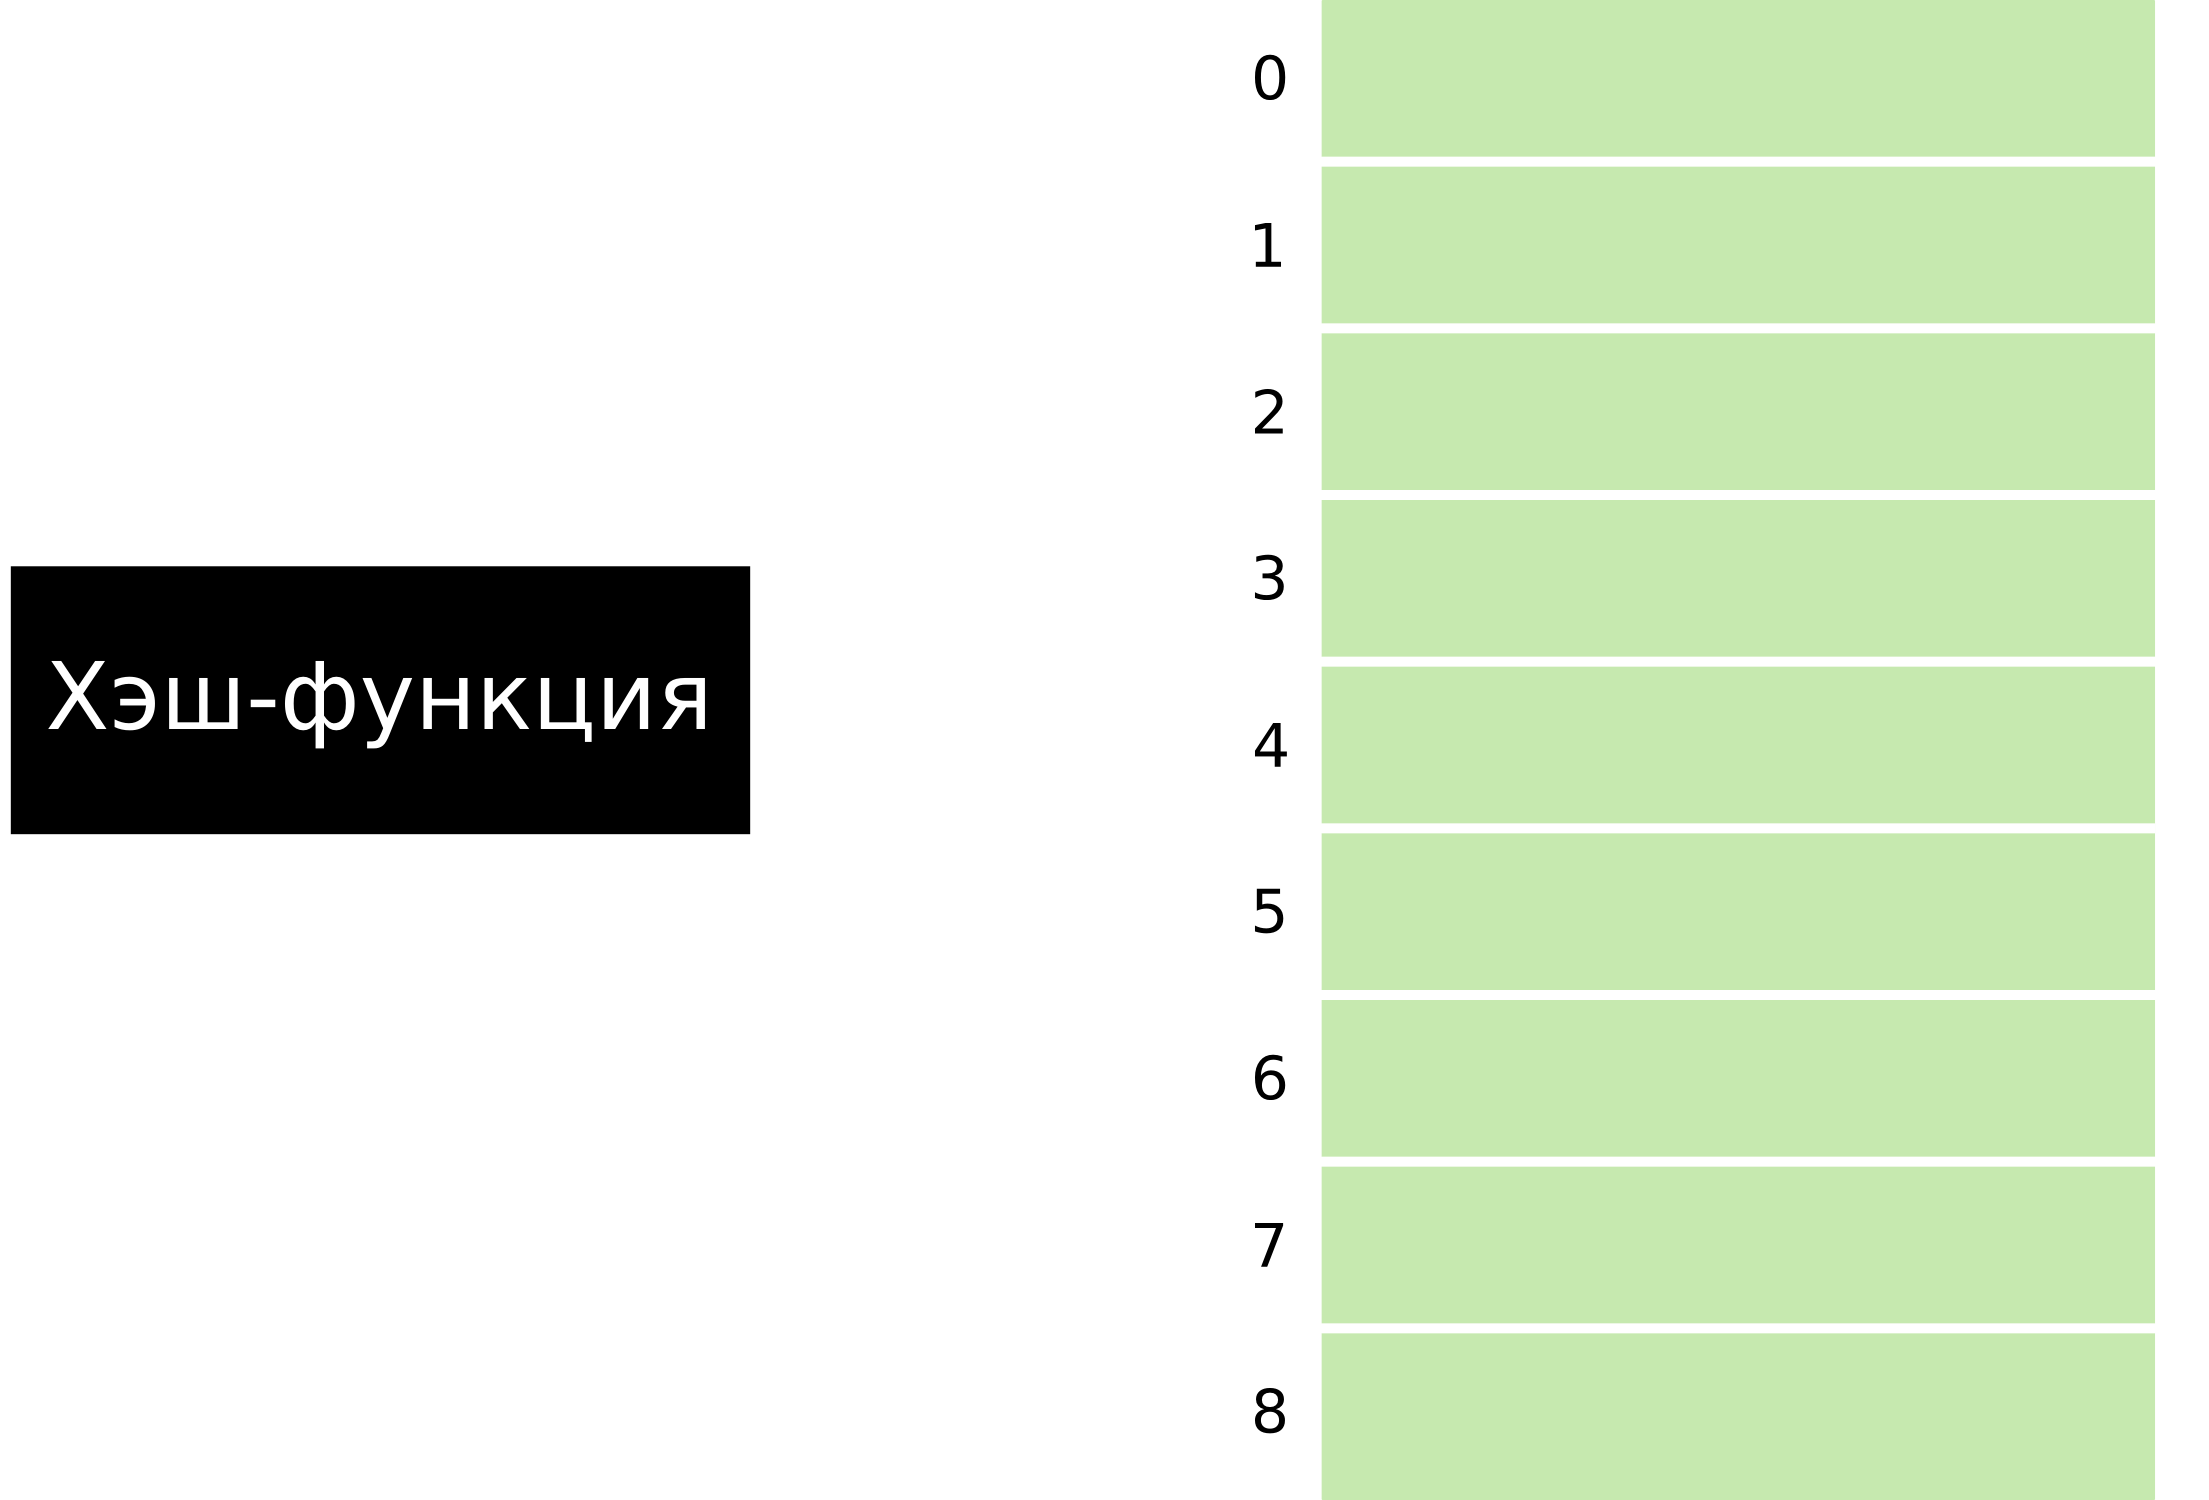
\includegraphics[width=0.86\linewidth]{images/hash_1.png}}
\end{figure}
\end{frame}

\begin{frame}{Хэш-таблица.}
\begin{figure}
\centerline{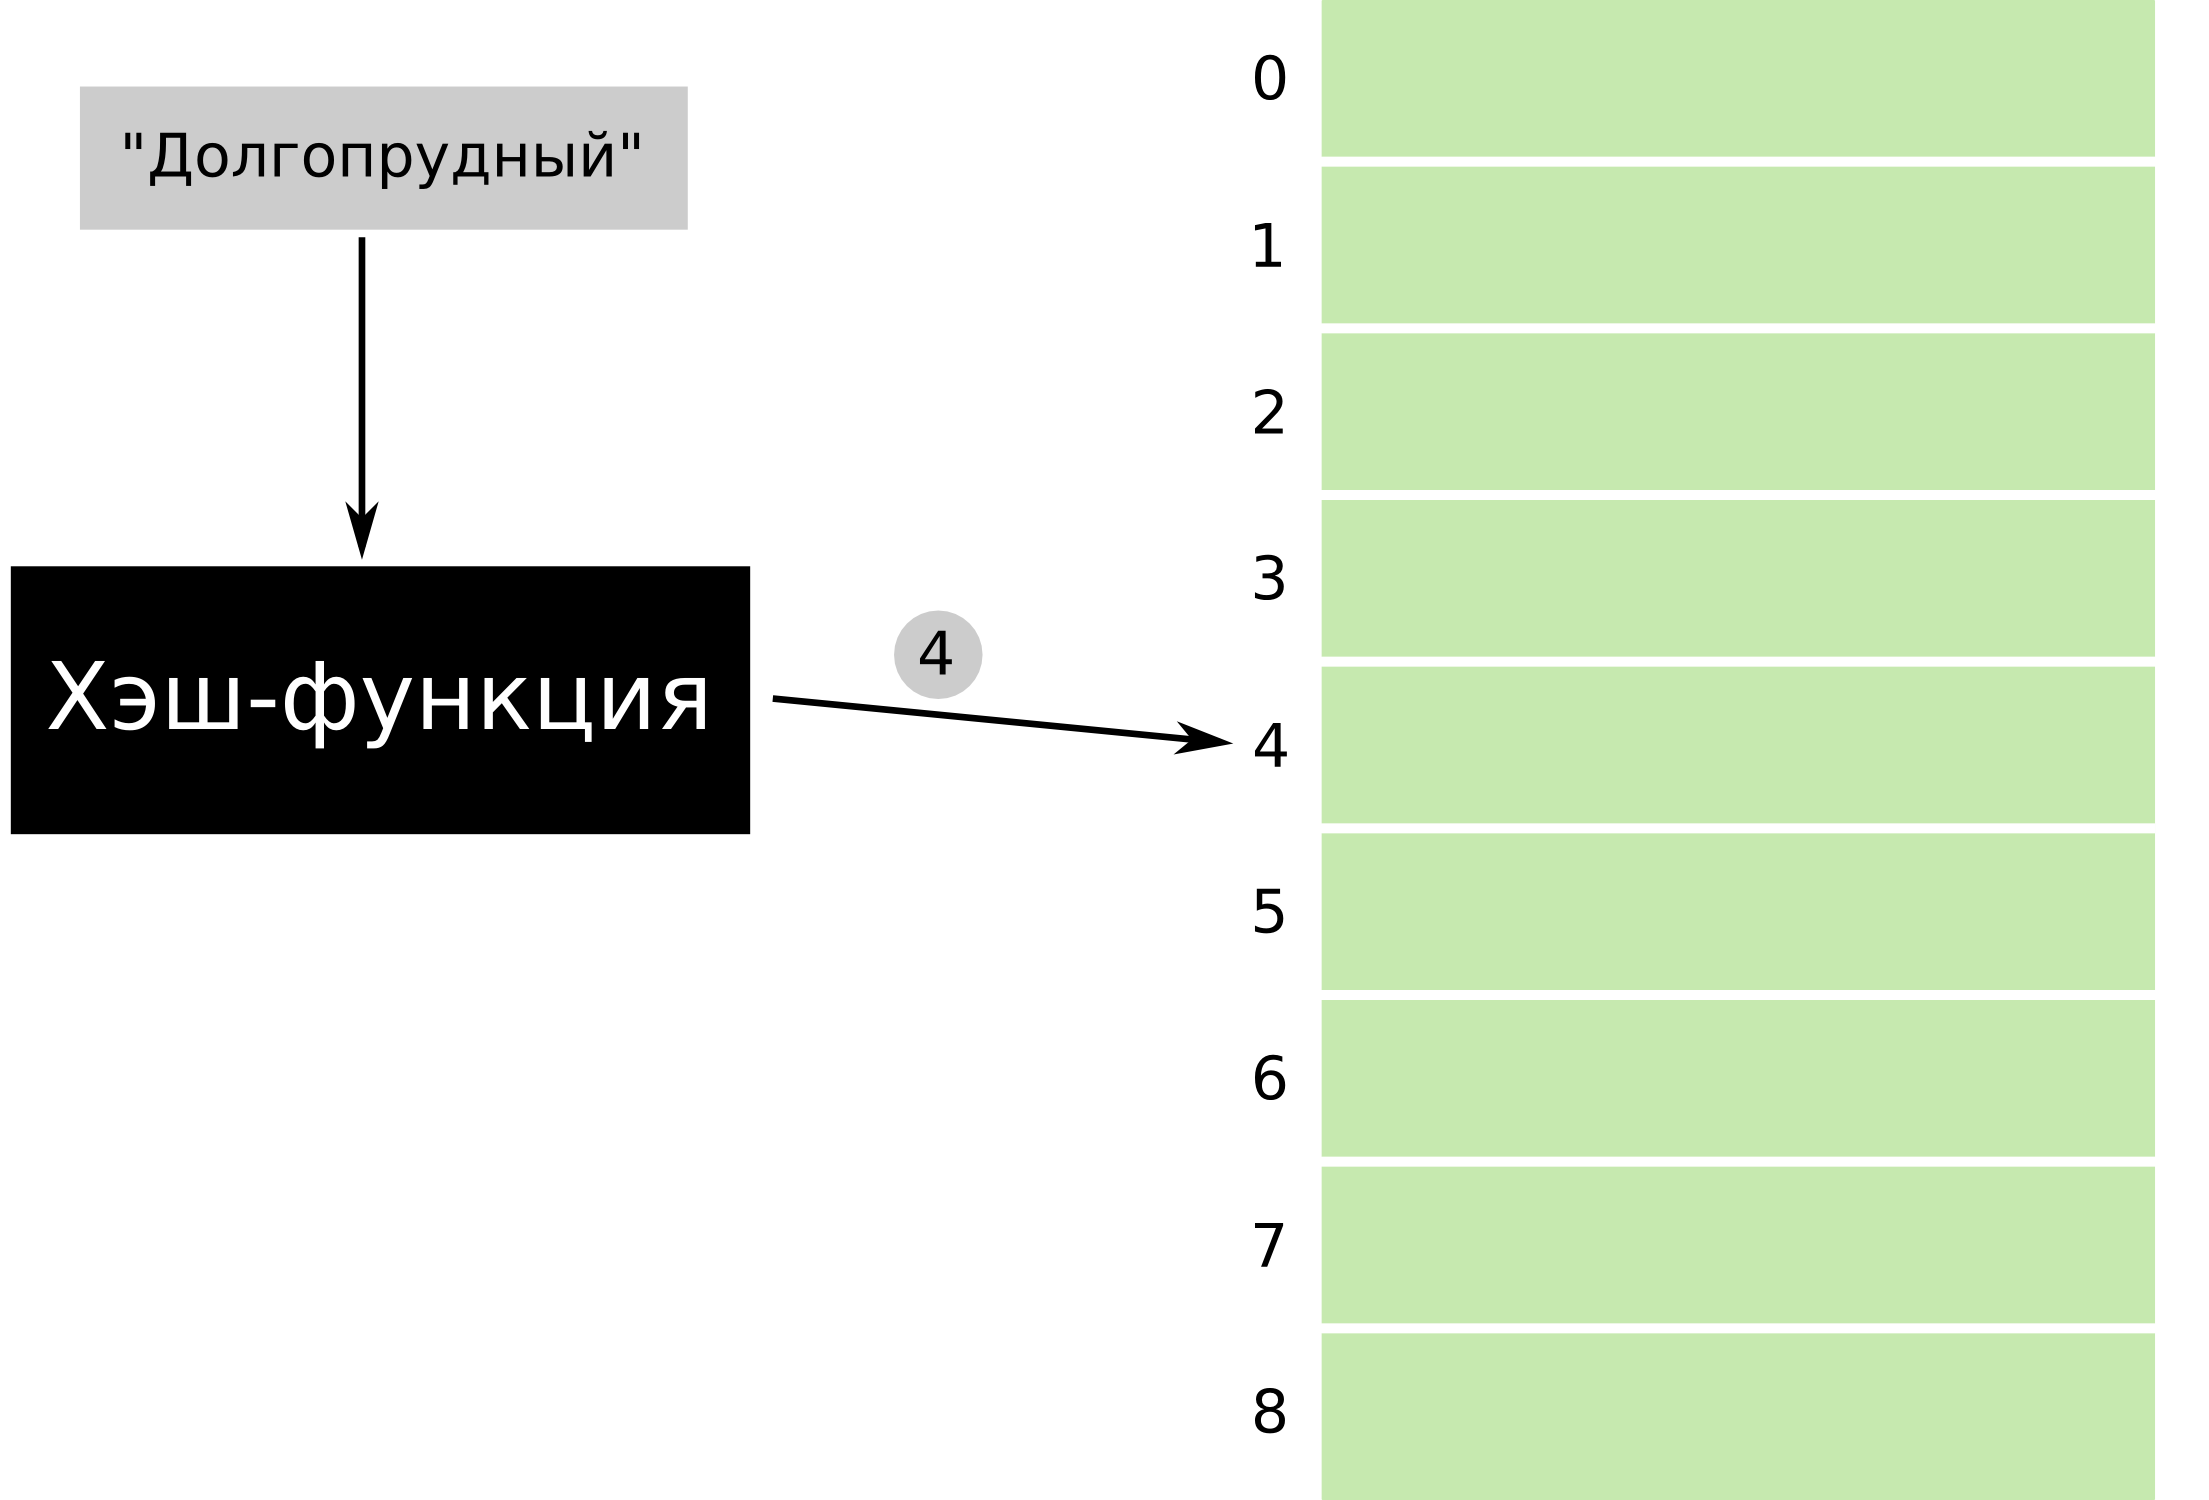
\includegraphics[width=0.86\linewidth]{images/hash_2.png}}
\end{figure}
\end{frame}

\begin{frame}{Хэш-таблица.}
\begin{figure}
\centerline{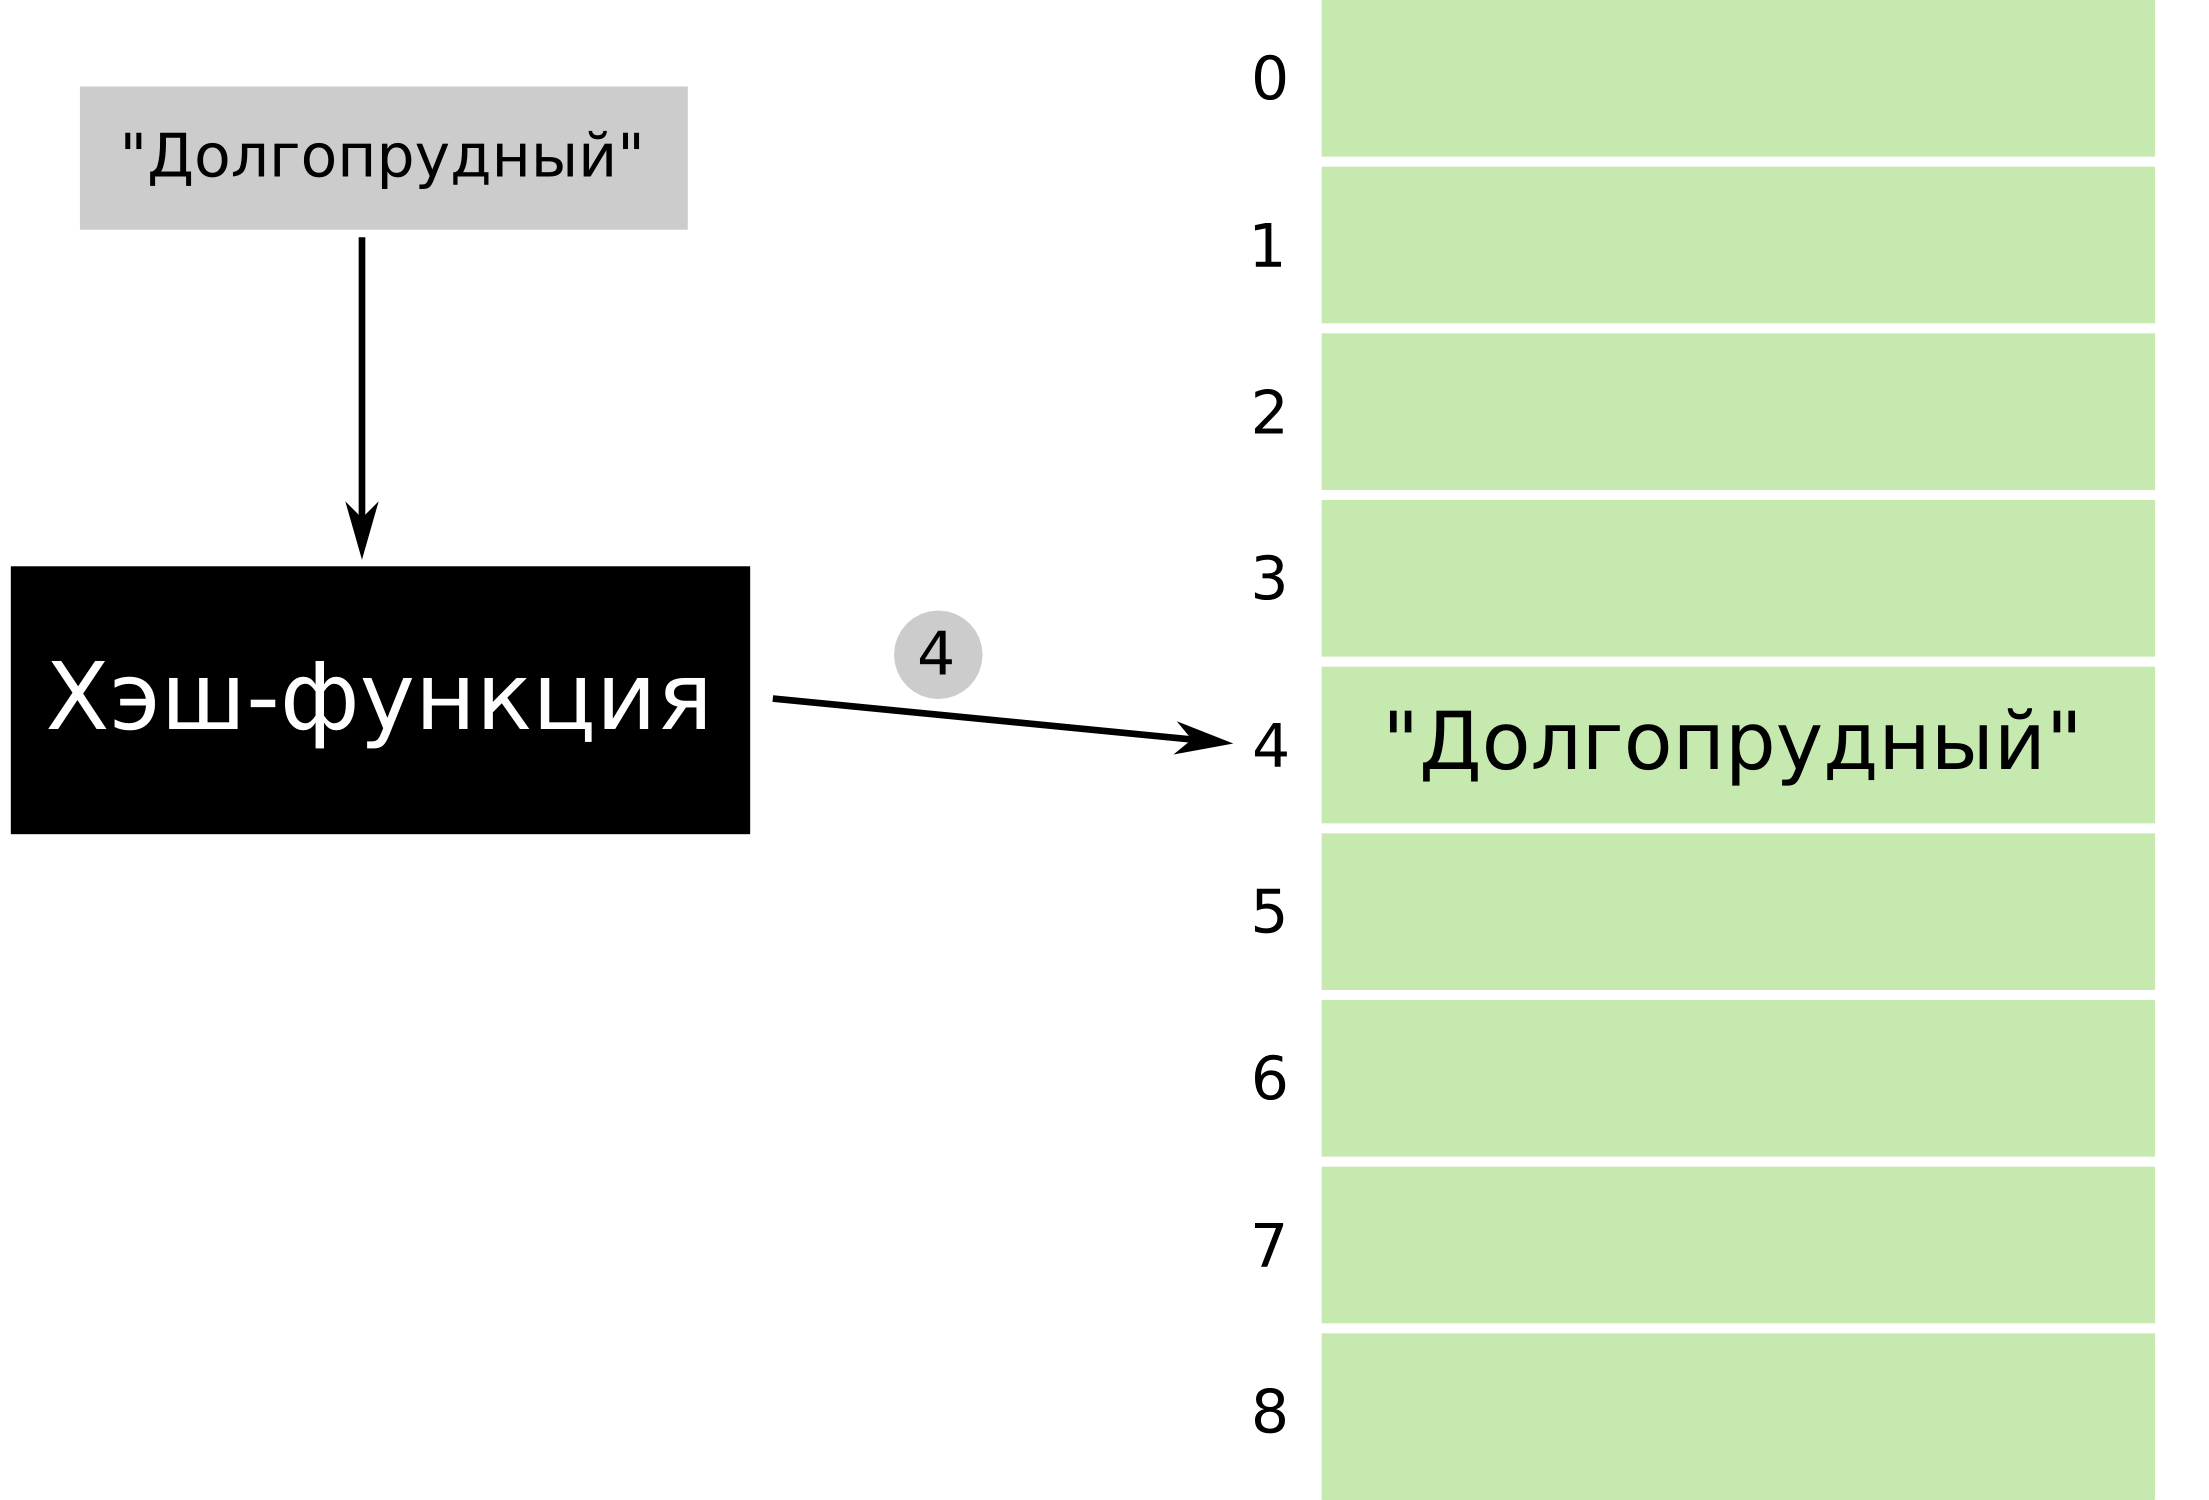
\includegraphics[width=0.86\linewidth]{images/hash_3.png}}
\end{figure}
\end{frame}

\begin{frame}{Хэш-таблица.}
\begin{figure}
\centerline{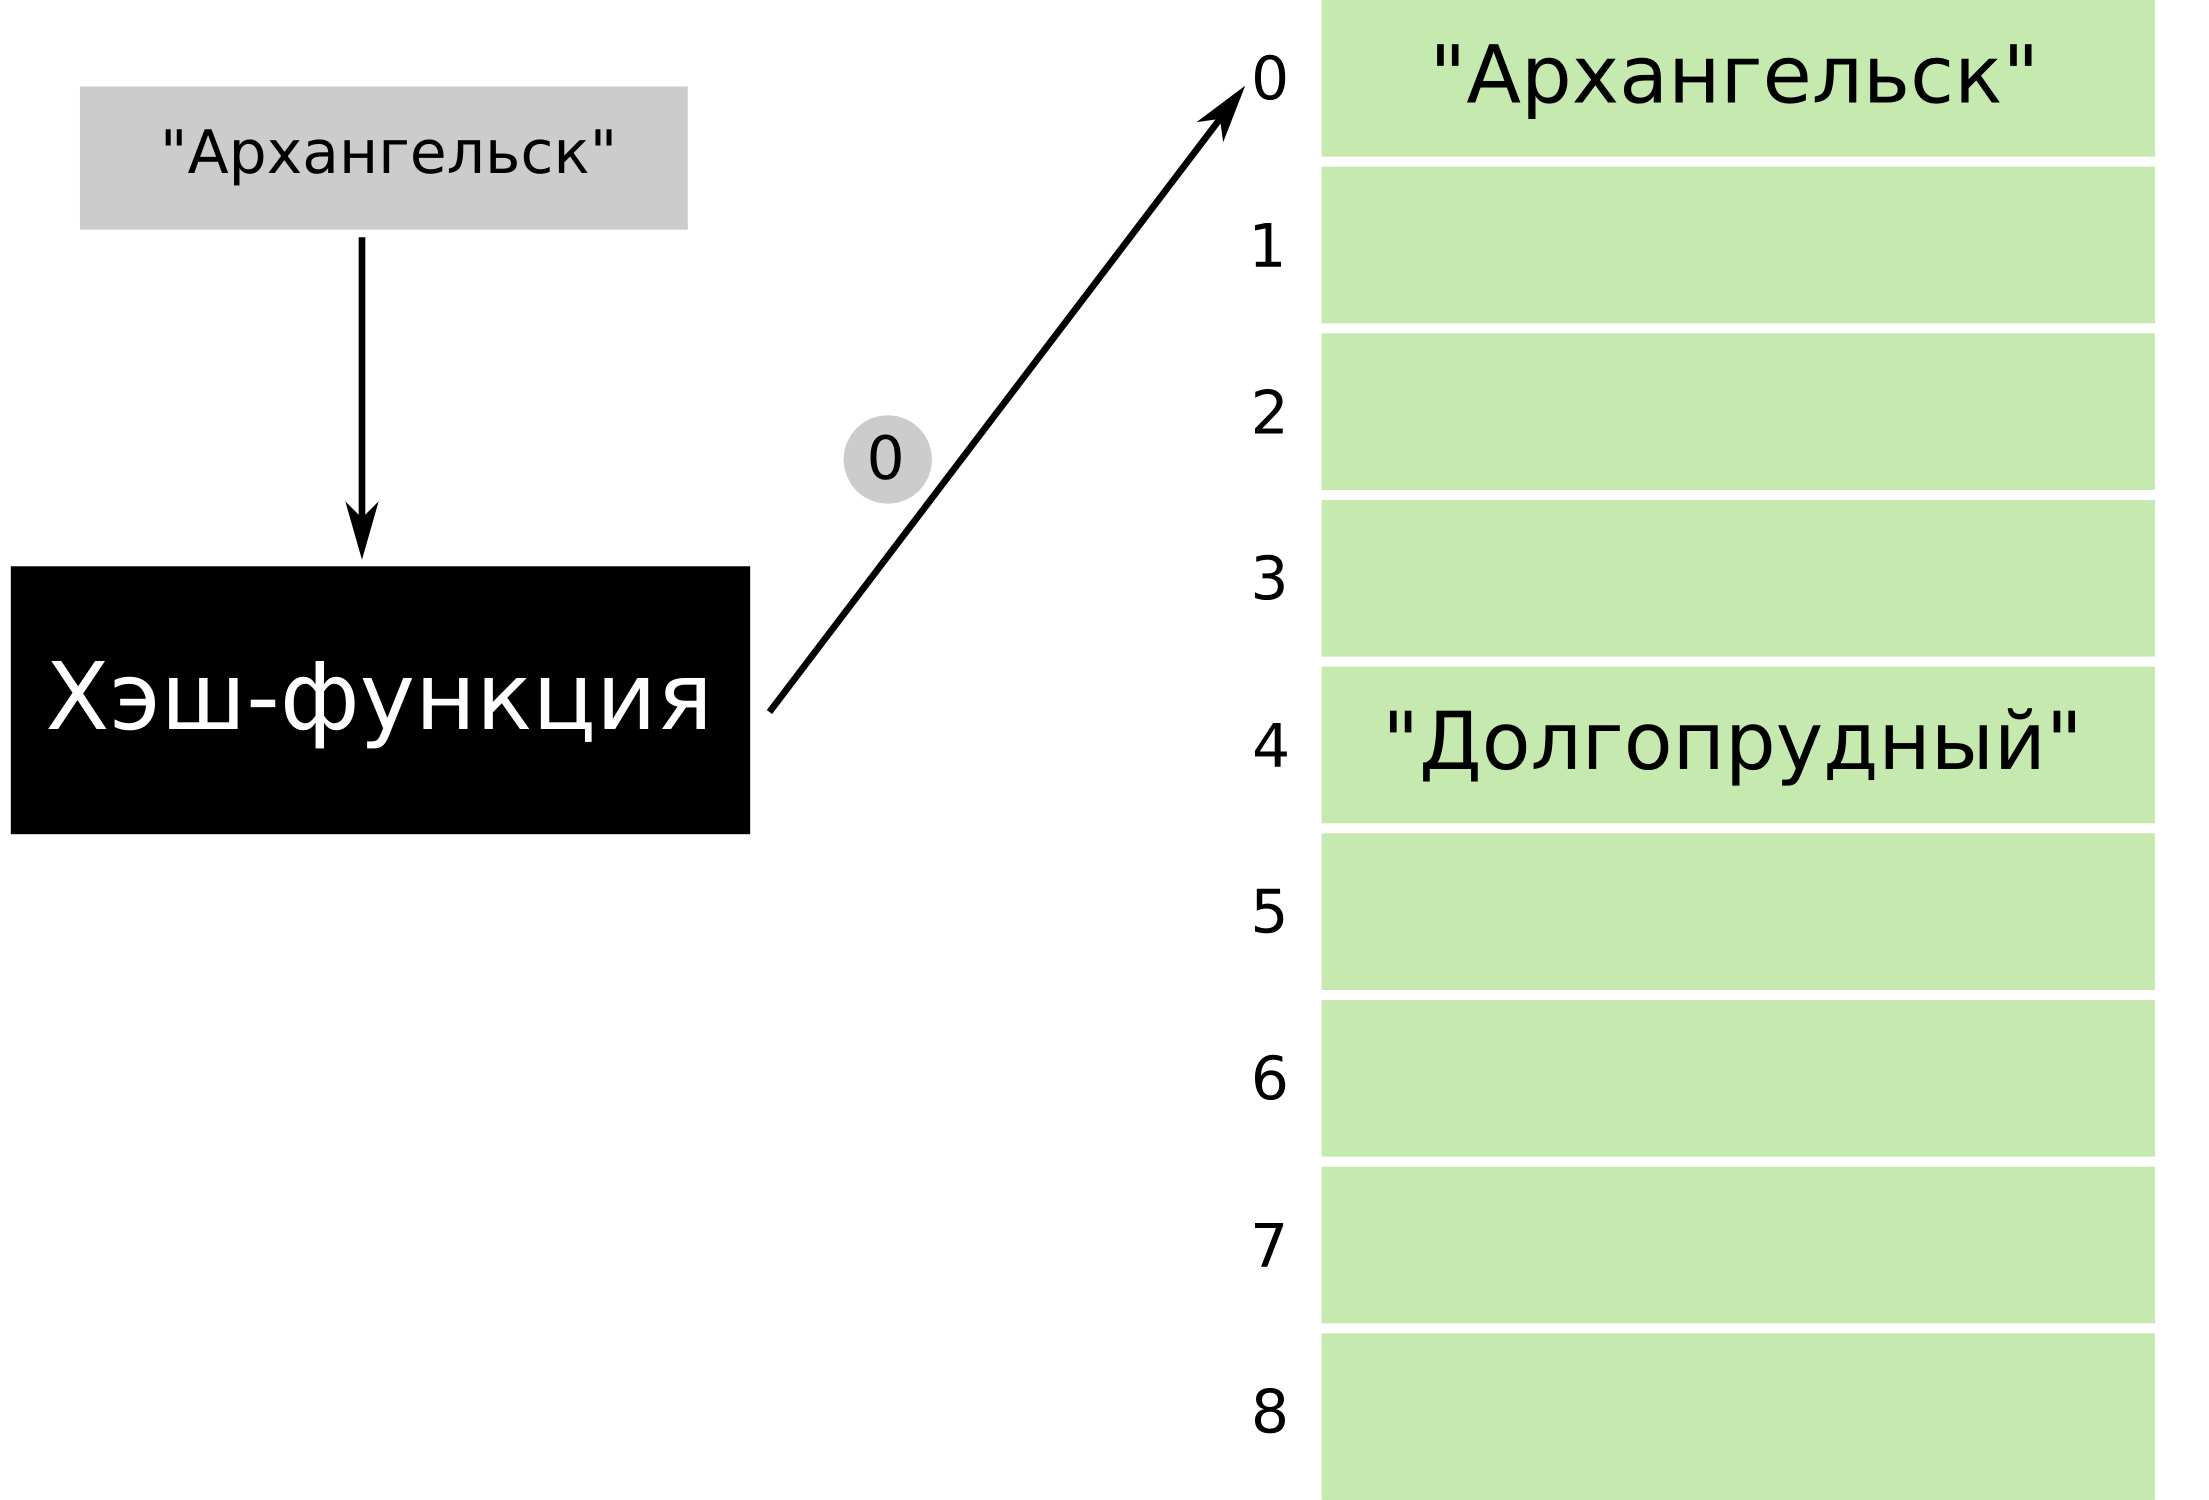
\includegraphics[width=0.86\linewidth]{images/hash_4.png}}
\end{figure}
\end{frame}

\begin{frame}{Хэш-таблица.}
\begin{figure}
\centerline{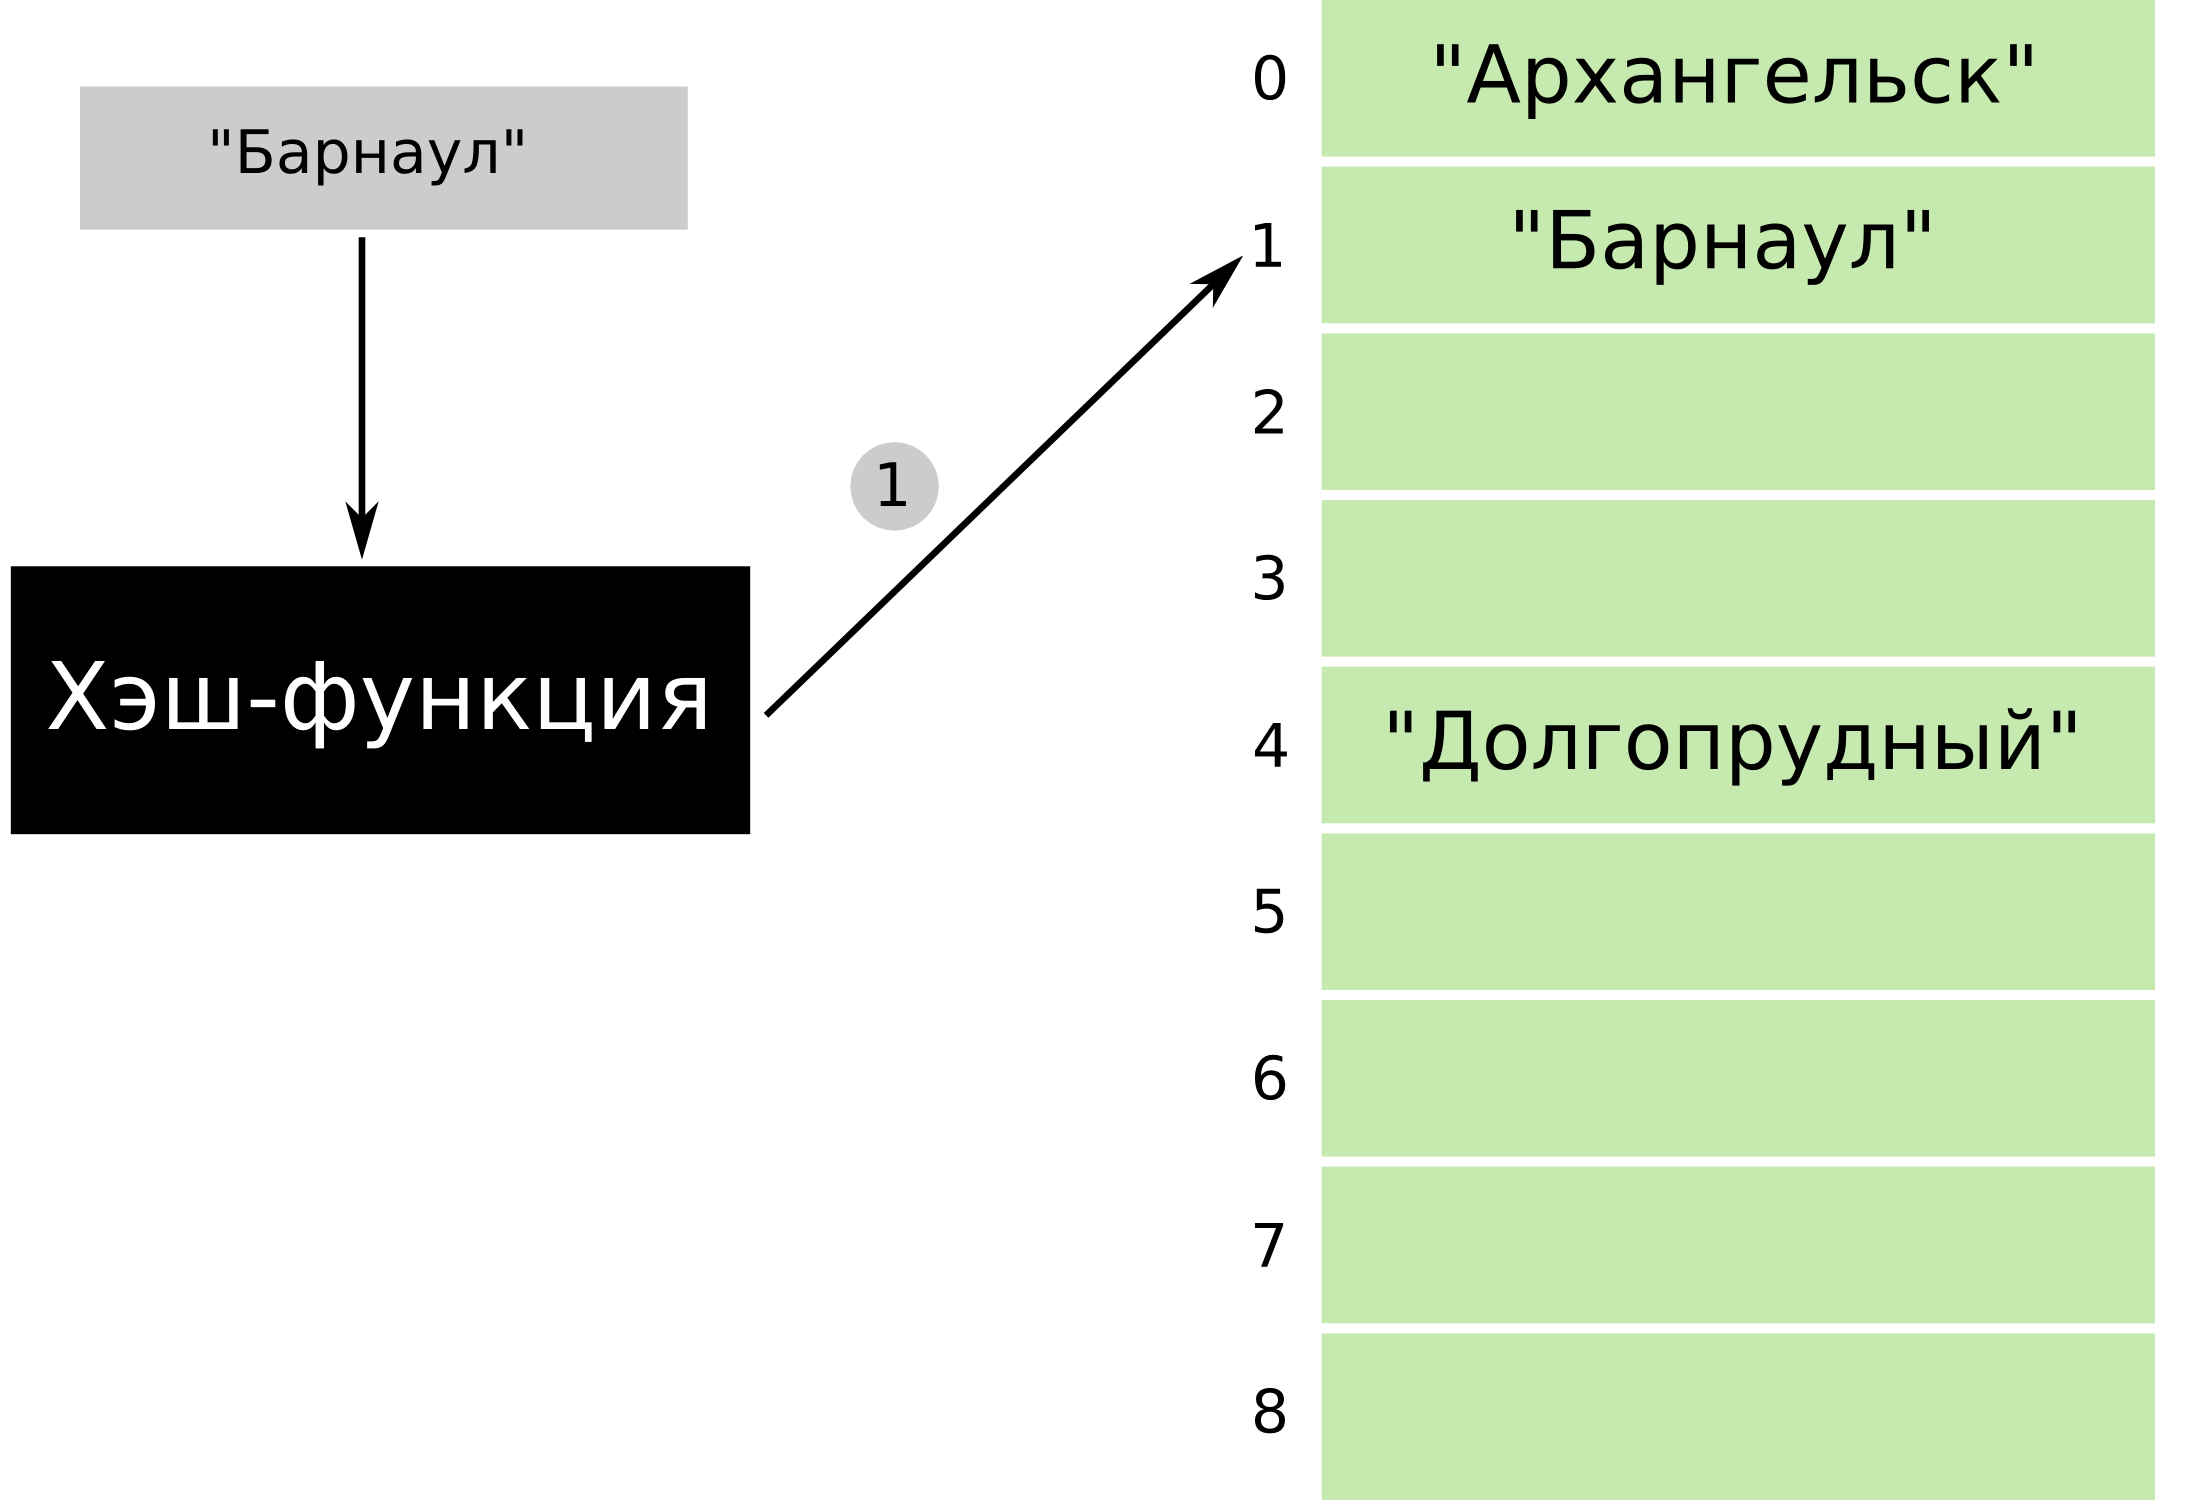
\includegraphics[width=0.86\linewidth]{images/hash_5.png}}
\end{figure}
\end{frame}

\begin{frame}{Хэш-таблица.}
\begin{figure}
\centerline{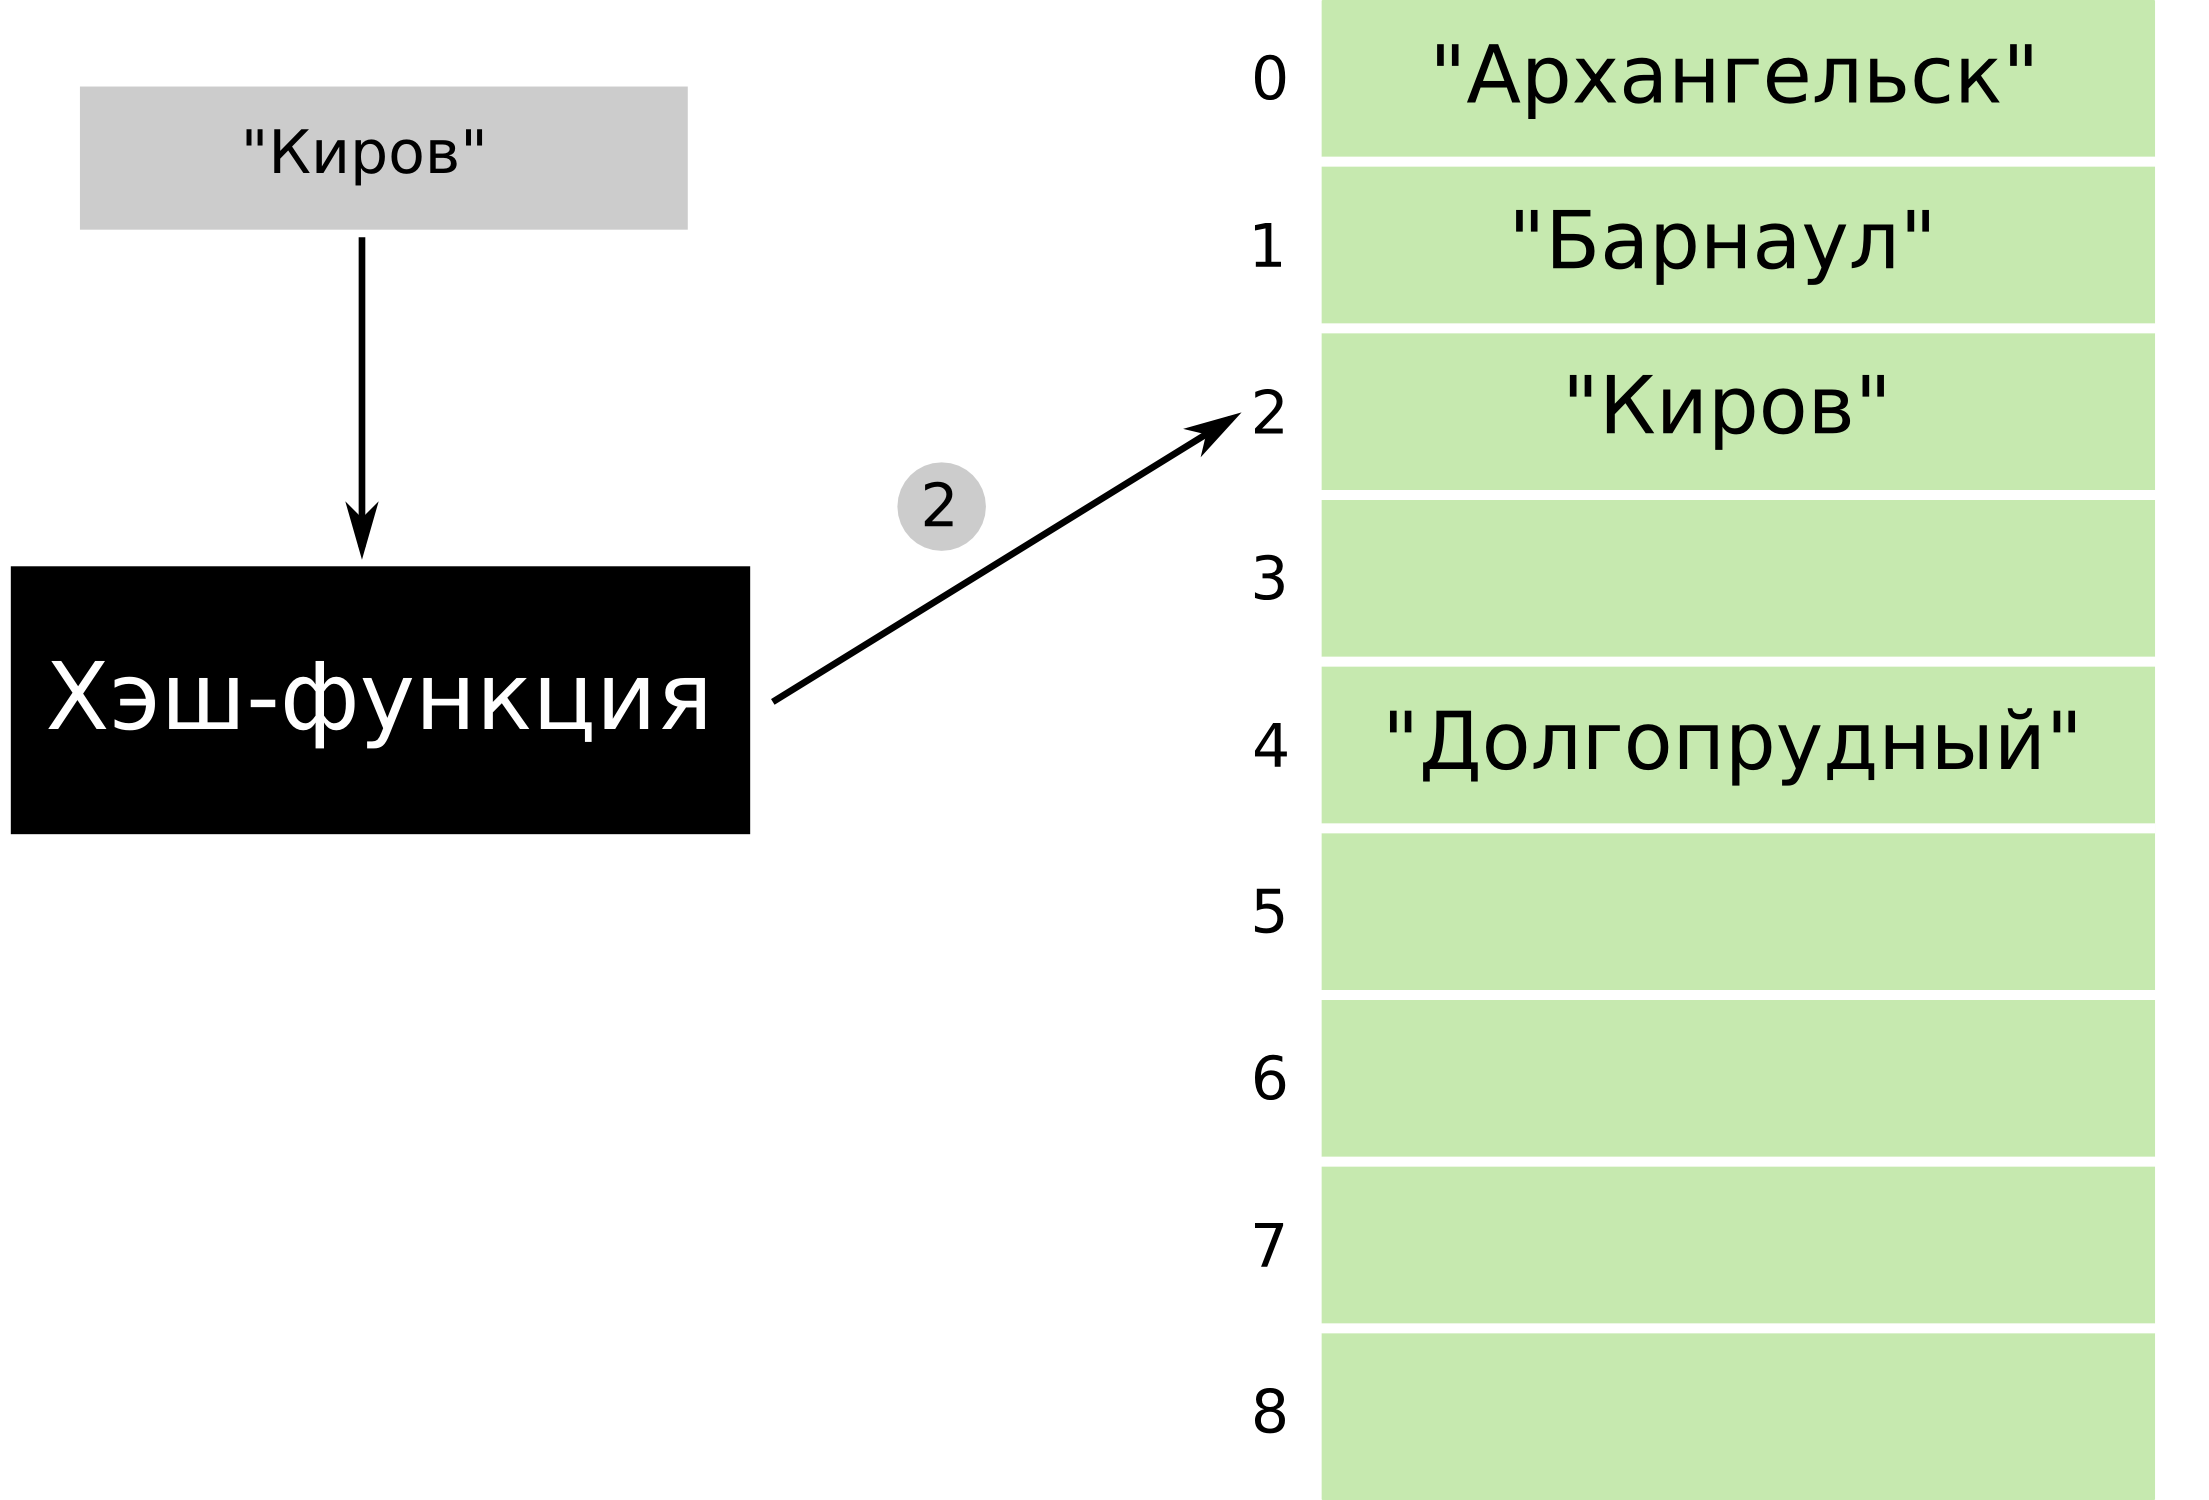
\includegraphics[width=0.86\linewidth]{images/hash_6.png}}
\end{figure}
\end{frame}

\begin{frame}{Хэш-таблица.}
\begin{figure}
\centerline{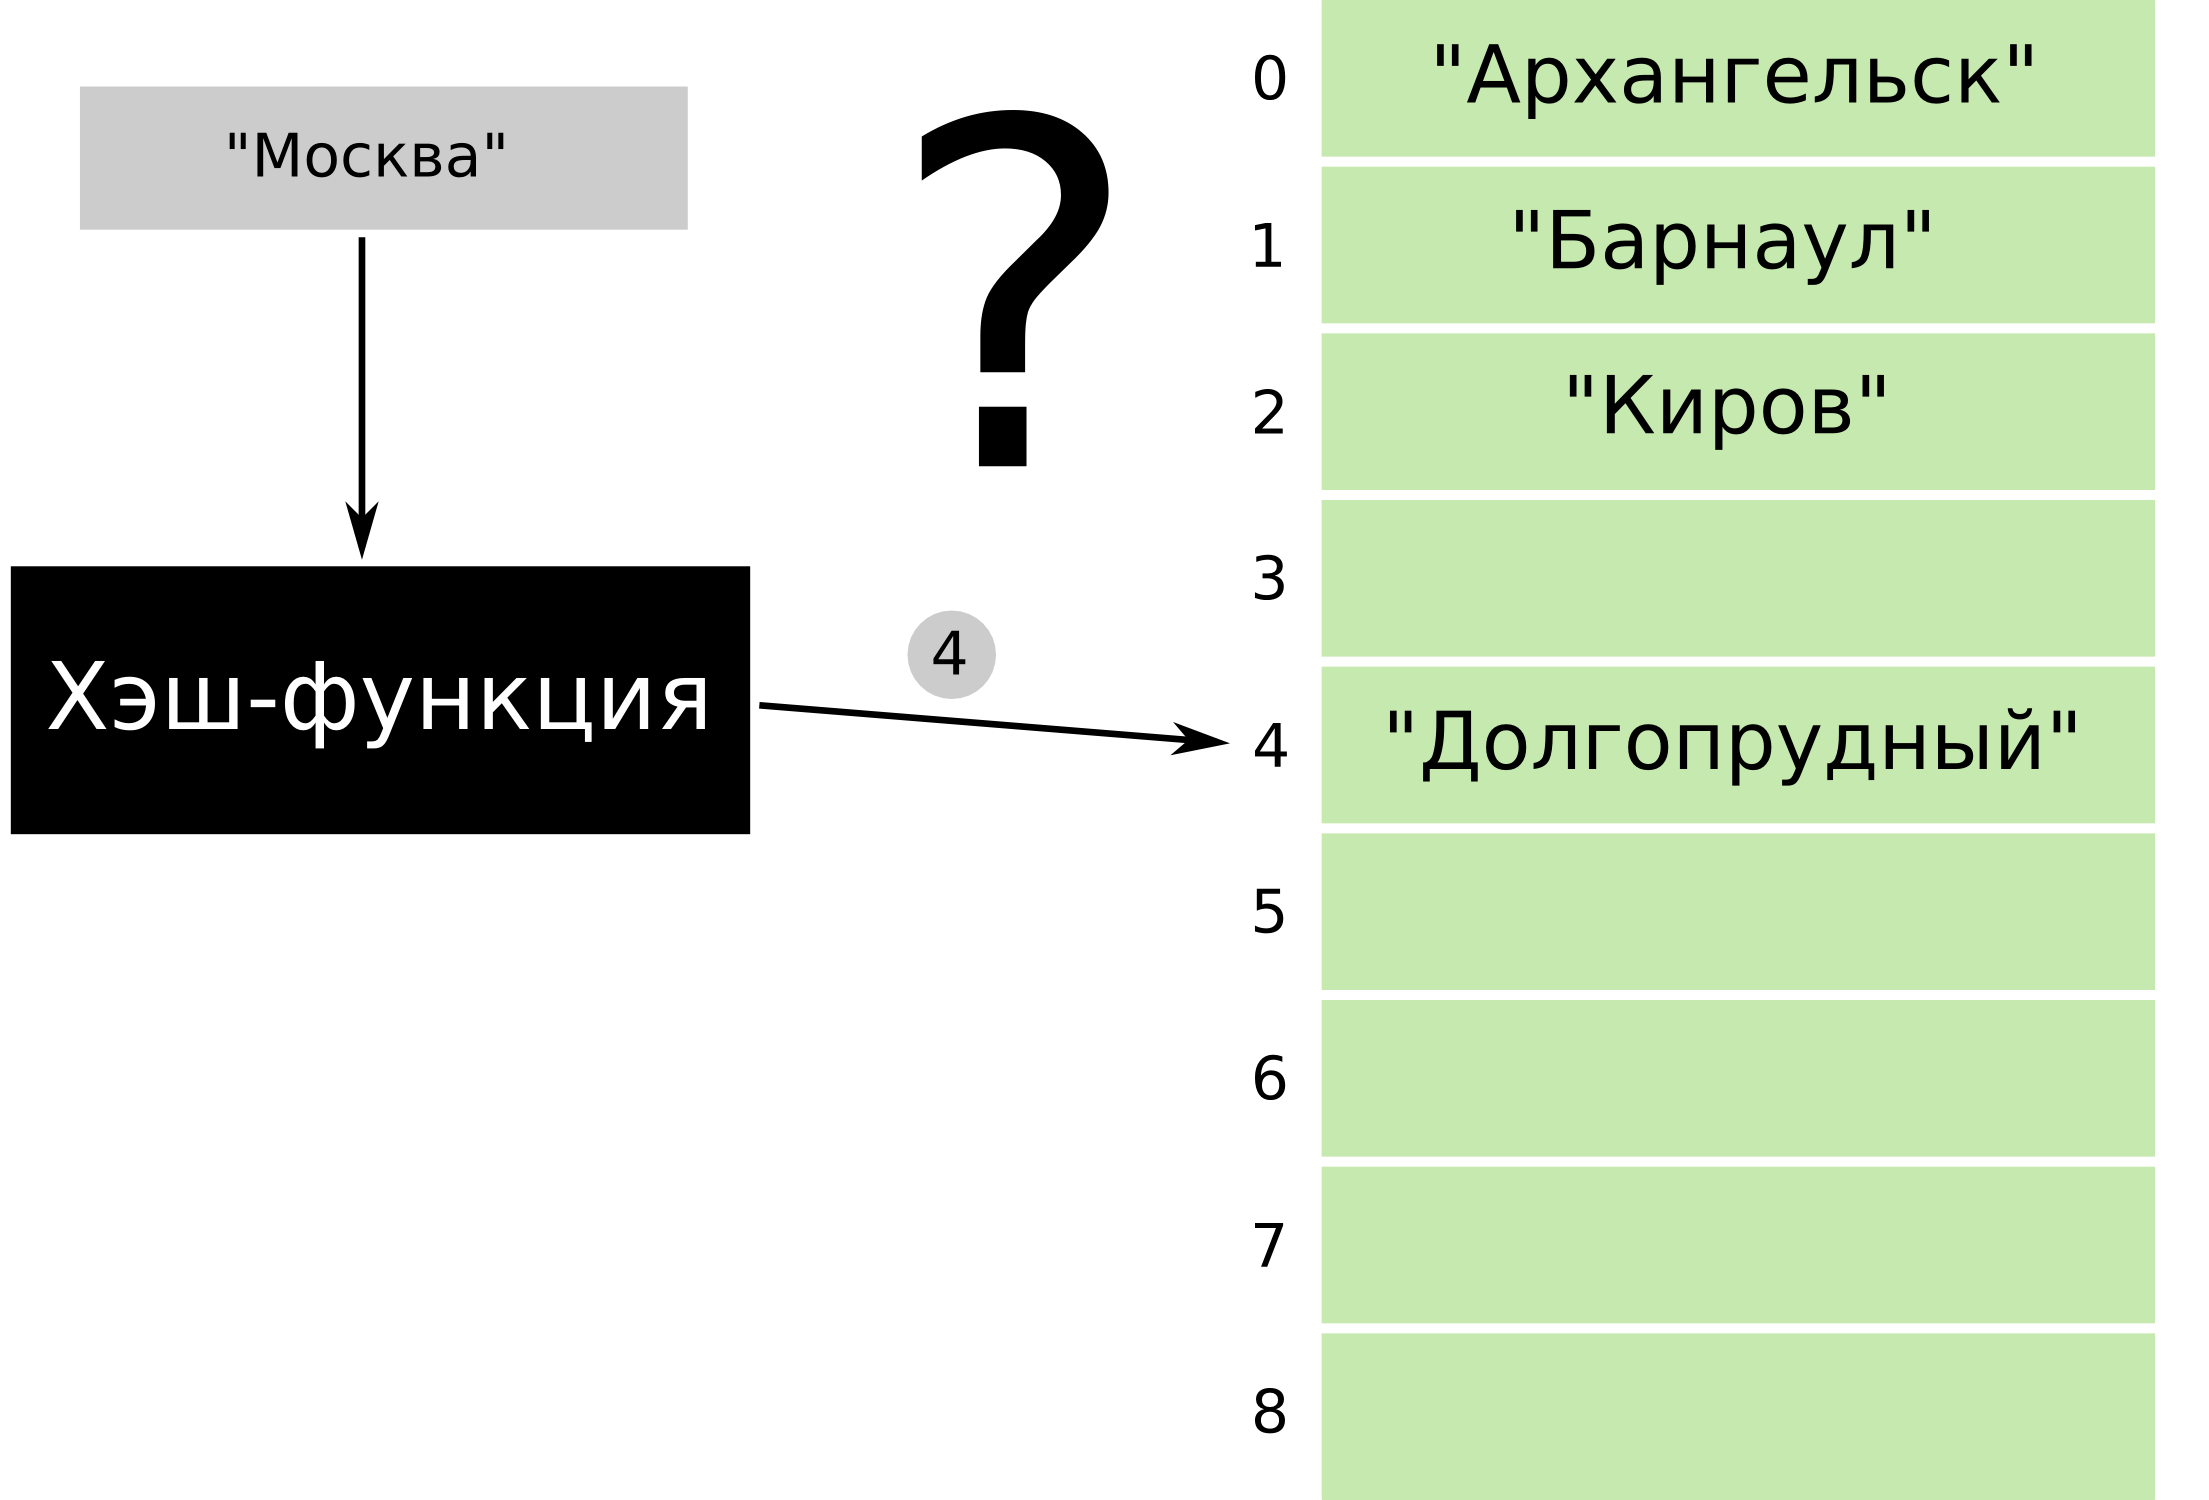
\includegraphics[width=0.9\linewidth]{images/hash_7.png}}
\end{figure}
\end{frame}

\begin{frame}{Хэш-таблица.}
\begin{figure}
\centerline{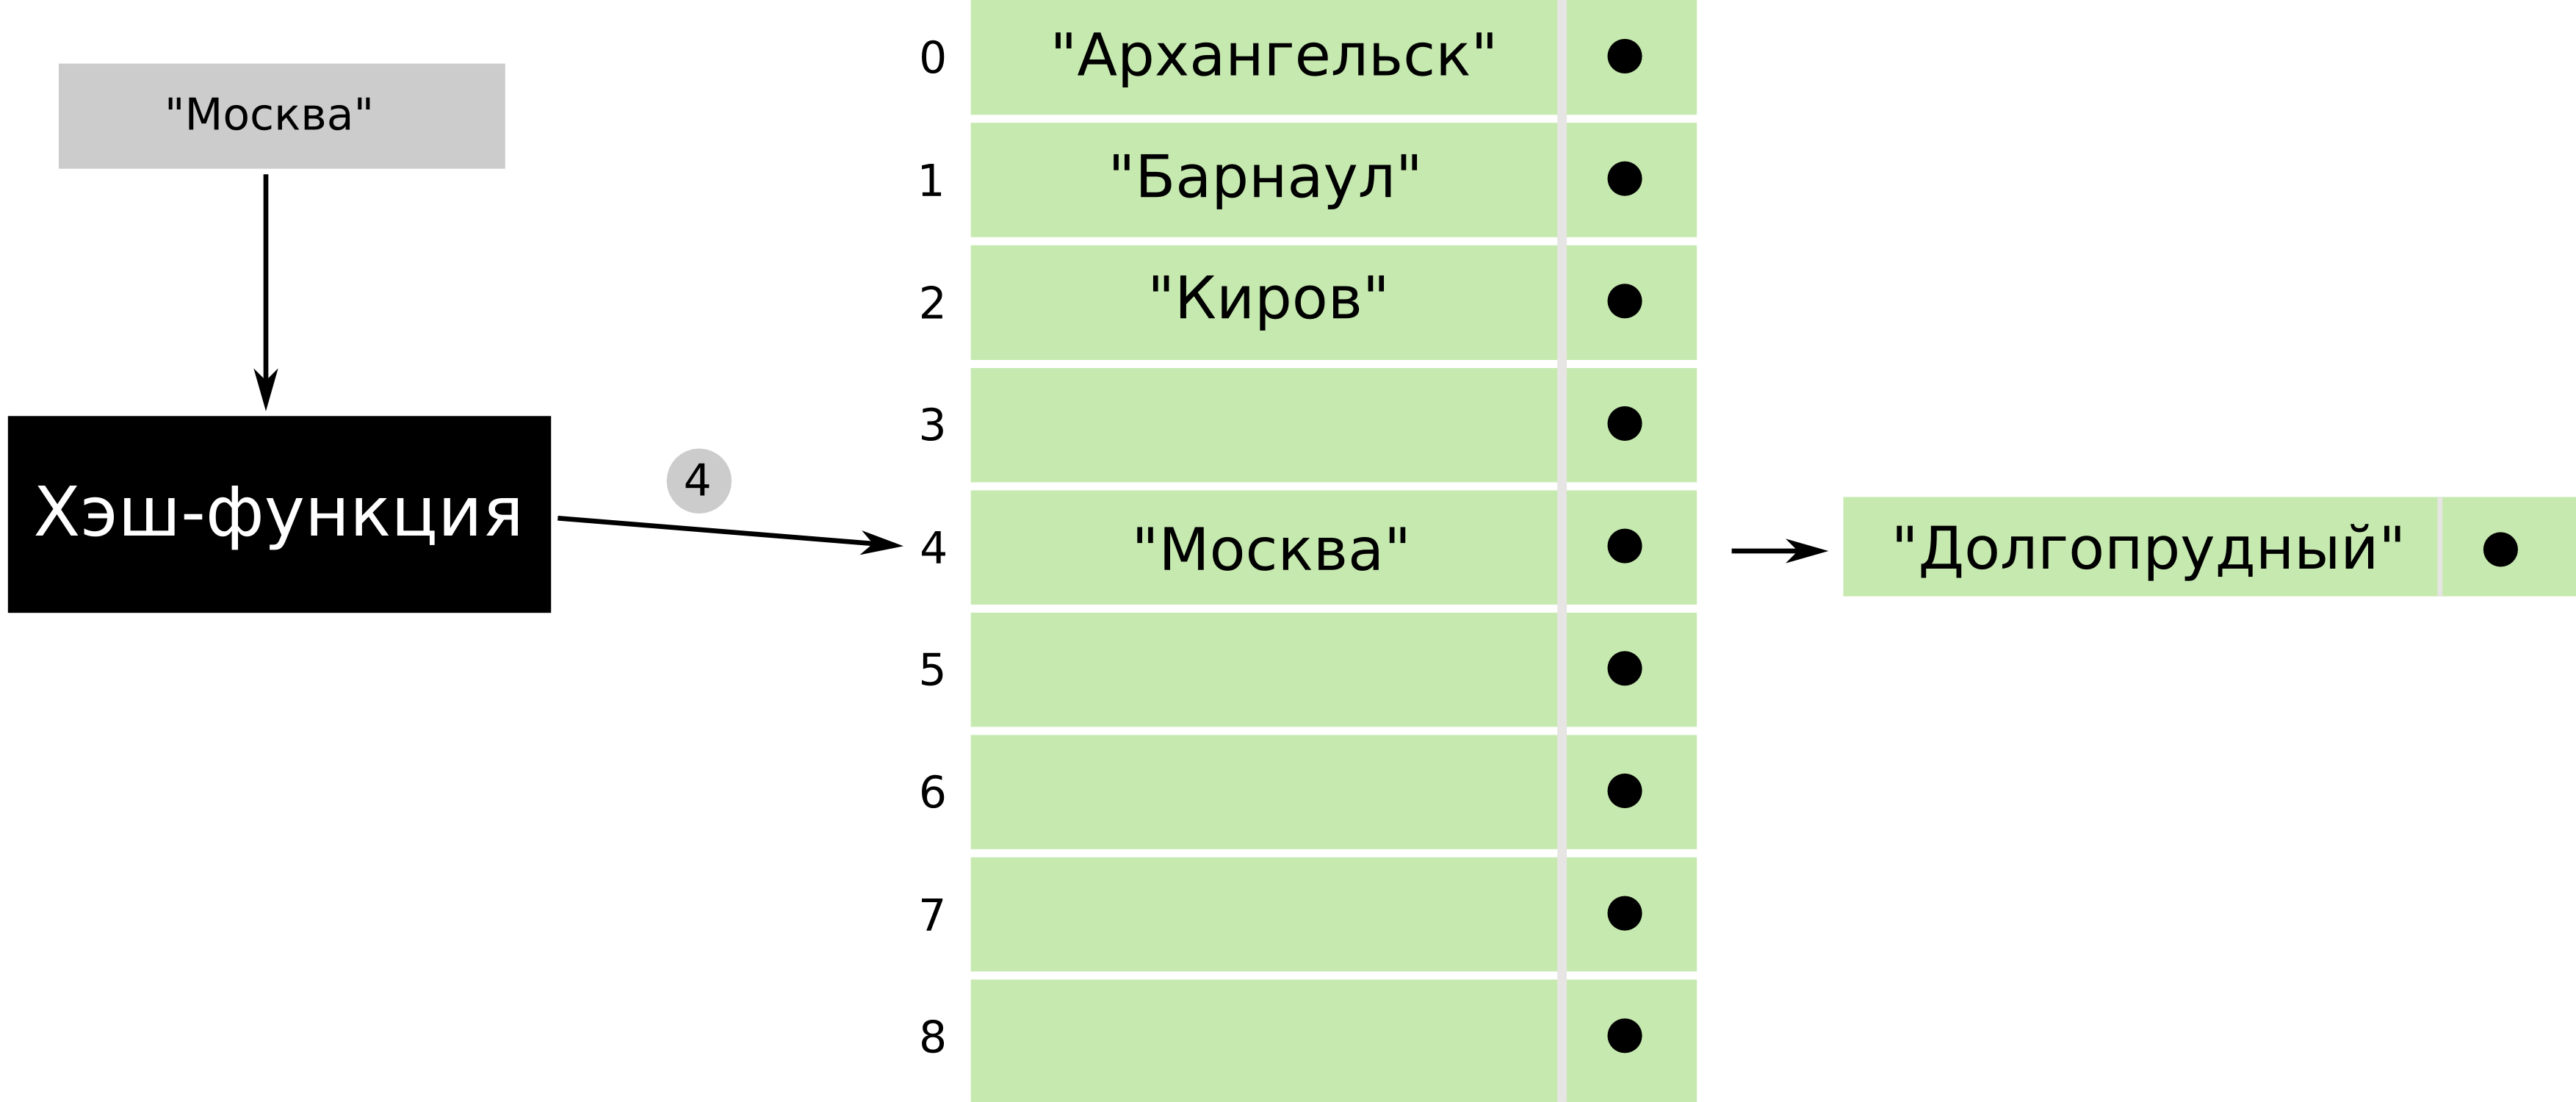
\includegraphics[width=0.99\linewidth]{images/hash_8.png}}
\end{figure}
\end{frame}

\begin{frame}{Хэш-таблица.}
\begin{figure}
\centerline{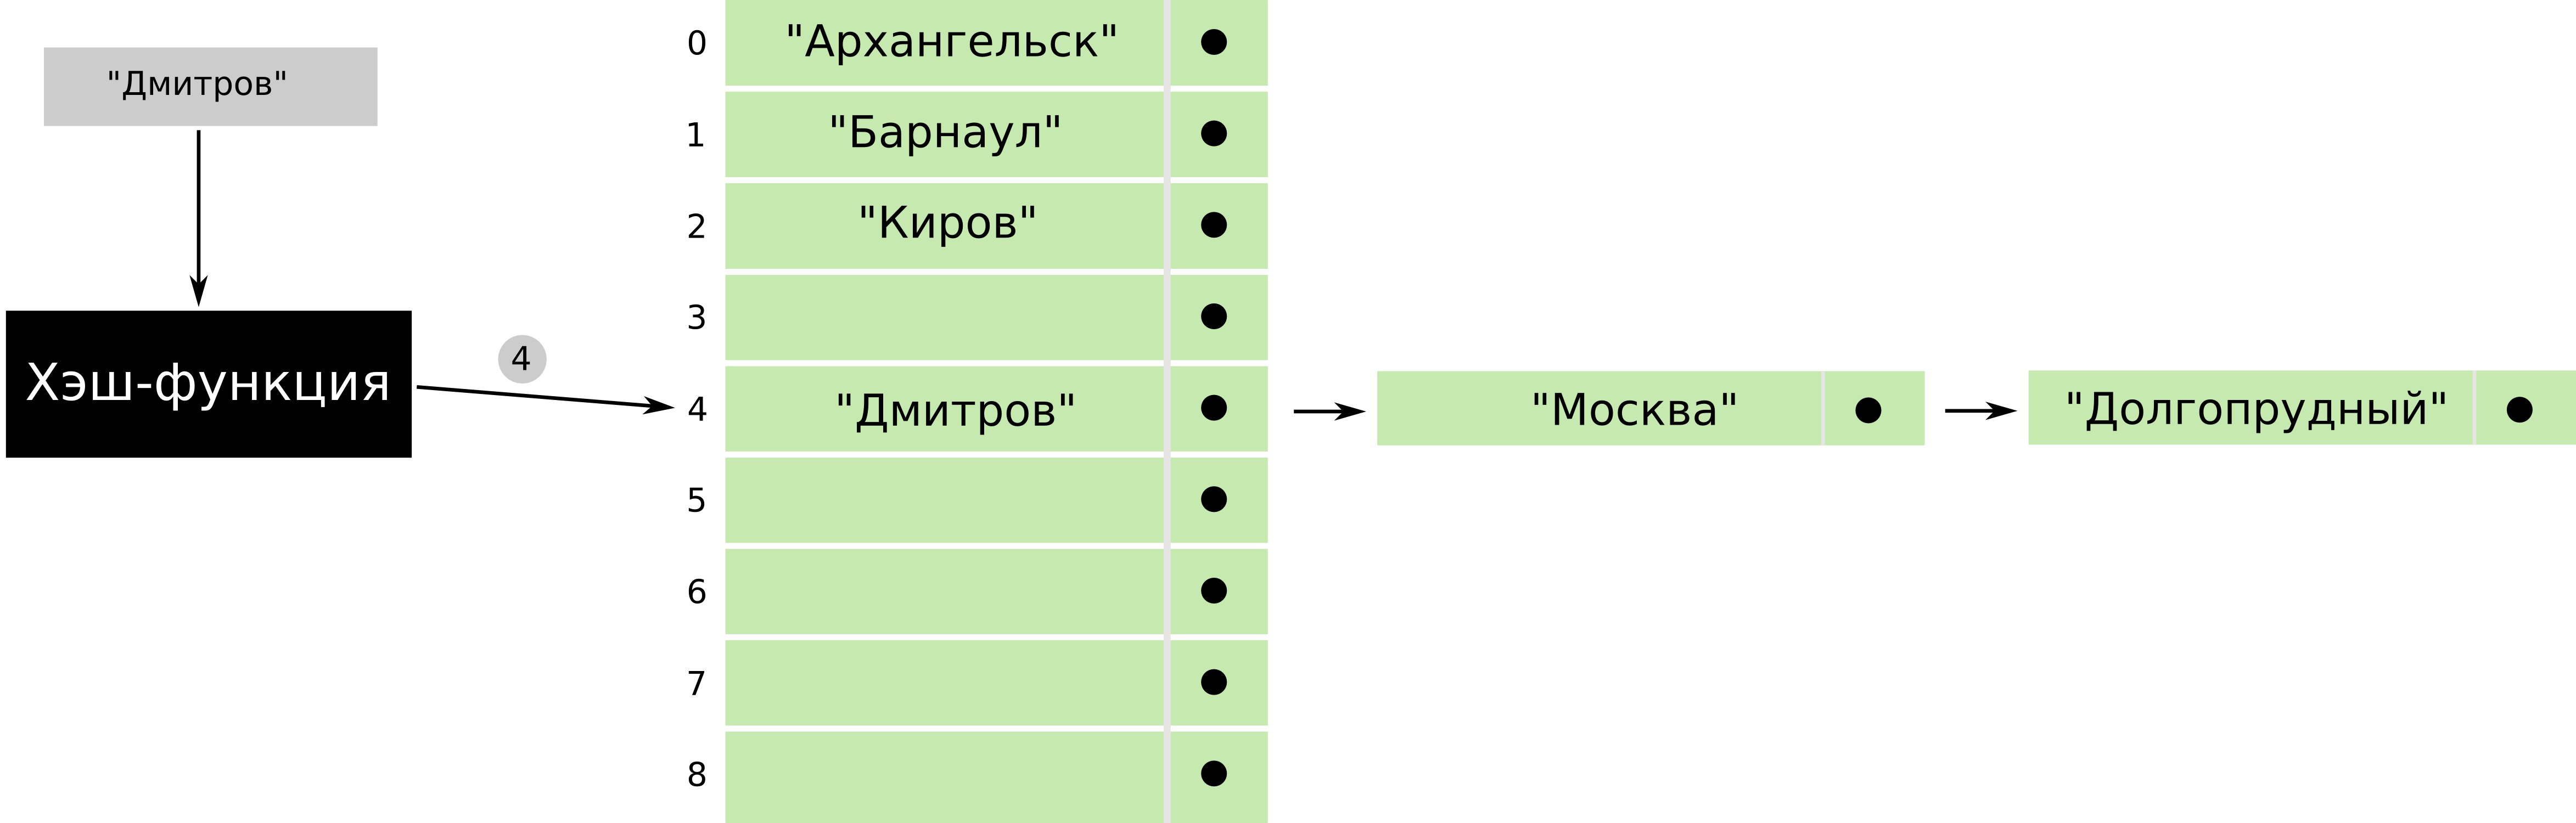
\includegraphics[width=0.99\linewidth]{images/hash_9.png}}
\end{figure}
\end{frame}



\begin{frame}{Граф. Сложности работы алгоритмов.}
\begin{itemize}
\item BFS -- $O(|V| + |E|)$
\item DFS -- $O(|V| + |E|)$
\item Алгоритм Дейкстры -- $O(|V|^2 + |E|)$
\item Алгоритм Беллмана-Форда -- $O(|V|*|E|)$ \\
(алгоритм нахождения кратчайших путей из одной вершины если есть отрицательные веса)
\item Алгоритм Флойда-Уоршолла -- $O(|V|^3)$ \\
(алгоритм нахождения кратчайших путей для всех пар вершин)
\end{itemize}
\end{frame}

%-=-=-=-=-=-=-=-=-=-=-=-=-=-=-=-=-=-=-=-=-=-=-=-=
%	Practical part:
%-=-=-=-=-=-=-=-=-=-=-=-=-=-=-=-=-=-=-=-=-=-=-=-=


\section{Практическая часть}






\end{document}